


\documentclass[main]{subfiles}

\begin{document}


\chapter{Results \& Insights}


This chapter includes the saliency metric and qualitative results from testing the method panel on ImageNet data and pre-trained CNN models. Insights on each method are compared with existing insights in the literature and summarised at the end of the chapter.

\section{Results Overview}

\subsection{Sample Sizes}  \label{sec:data_collection}
A set of 300 attributions for the full method panel took around 10 hours to collect and evaluate using a Nvidia GTX-1080 GPU. LIME was thought to be a key bottleneck due to its perturbation-based approach, but analysis in Section \ref{sec:perform} showed GradCAM was also slow in attribution. After several hundred attributions the process also became very slow and would have to be restarted from that point (possibly due to a GPU memory leak in method internals). These performance considerations meant only 1000 instances out of 50,000 available in the validation set were used for evaluation. This was at least the same 1000 instances for all methods, and different dimensions were added to generate insights regardless: different attribution thresholds, and subsetting the results for high confidence (p $>0.9$) vs low confidence model predictions.

\subsection{Software Availability}

Code for the project is available on GitHub and is intended to be made public after improving the existing model agnosticity for practitioners as well as cleaning up dependencies and file structures. The framework has modular support for attribution methods provided they are compatible with image data and return an input-space representation of their explanation, and modular support for other saliency metrics as mentioned in Section \ref{sec:sw3}.


\subsection{Other Model Testing} \label{sec:shap_note}

Some limitations were encountered on SHAP for ResNet50 and InceptionV3 architectures. Other methods were successfully tested on other models with results below, though the bug in SHAP was not resolved in time for project completion. The impact of this obstacle is discussed.

\section{Saliency Metric Results}
\subsection{VGG-16} \label{sec:vggExp}

Figure \ref{vggAfig} shows IOU and IOU* statistics for a 1000-instance sample explaining VGG-16 model predictions. The 1000 instances are broken up into high confidence (top row) and low confidence predictions (bottom row), where high confidence refers to a model output of $p>0.9$. Error bars indicate one standard deviation from the mean result displayed by bar height, and can be used a proxy of method consistency. For this setup a threshold of 0.5 standard deviations was applied to the attribution output for IOU and 1 standard deviation for IOU*.\\

\vspace{0.2in}
Some observations on Figure \ref{vggAfig} (other insights in Section \ref{sec:saliency_insights}):
\begin{itemize}
\item Results are similar for high vs low confidence predictions, with LIME's variance being one noticeable difference.
\item SHAP and DeepLift perform similarly on IOU but not IOU*
\item GradCAM scores lower on these metrics though is visually less noisy than DeepLIFT and SHAP
\end{itemize}


\newpage

%\vspace{2in}

\begin{figure}[h]\centering
\vfill
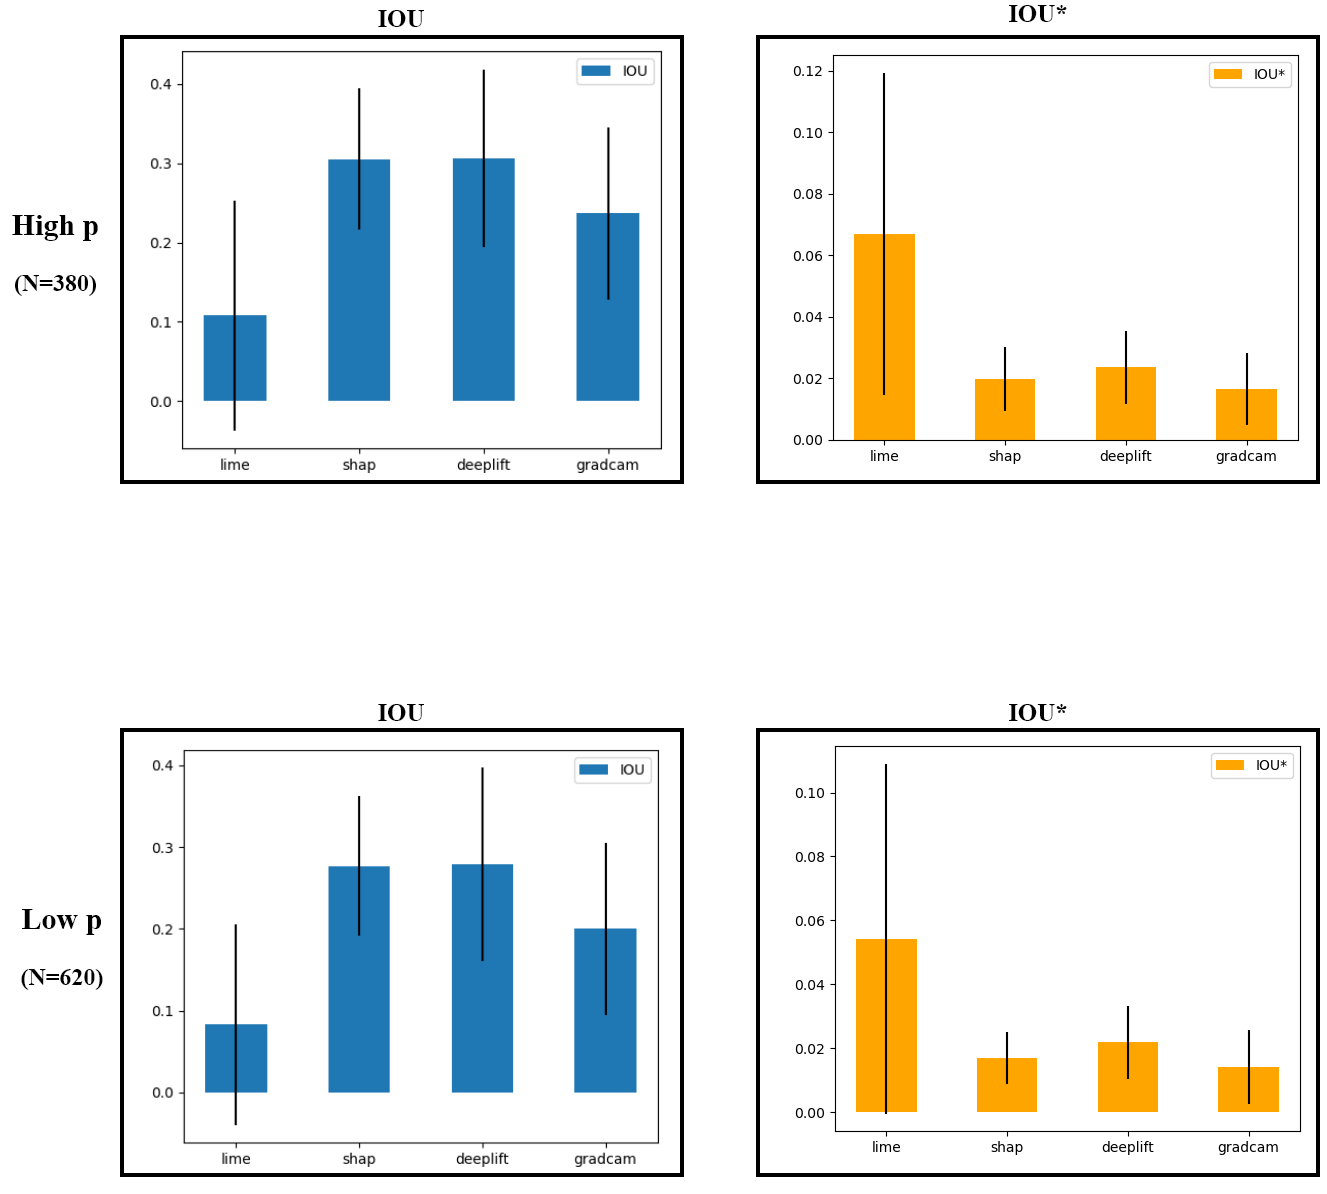
\includegraphics[scale=0.32]{vgg_0_5_and_1.png}
\caption{IOU, IOU* statistics for a 1000-instance attribution sample of VGG-16. }
\label{vggAfig}
\vfill
\end{figure}

In Appendix C, Figure X shows comparatively identical results for a smaller sample (N=300) with a different threshold set: 1 for IOU and 2 for IOU*.

\newpage



\subsection{InceptionV3}




\subsection{ResNet50}


\newpage
\subsection{Insights from Saliency Metrics} \label{sec:saliency_insights}


DeepLIFT performed strongly on VGG16 but poorly on more complex architectures.

Some results from the saliency metrics contradict visual observations from each method, however. This is explored in  For example, DeepLIFT's attributions were visually much noisier than others. Even with thresholds applied, it performed well on IOU possibly because of this noise across the input space.



What is it about the attribution weights that made IOU* high for DeepLIFT?? Why is GradCAM's variance higher??

\newpage
\section{Other Criteria}
\subsection{Performance} \label{sec:perform}


\begin{figure}[h]\centering
\vfill
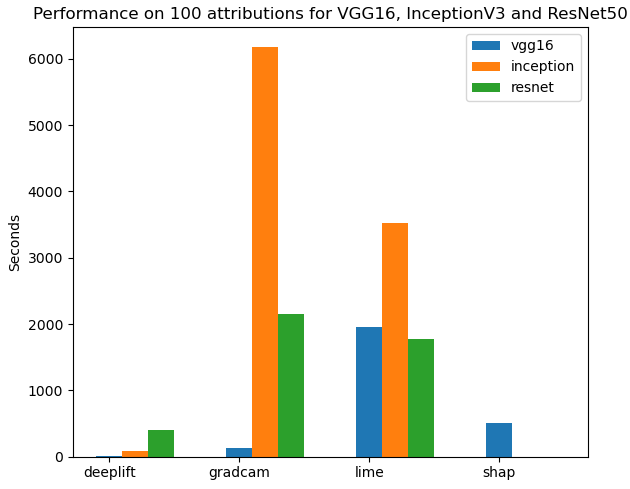
\includegraphics[scale=0.6]{performance.png}
\caption{Performance/speed in seconds for VGG-16, InceptionV3, and ResNet50. }
\label{performFig}
\vfill
\end{figure}

Some insights from performance measurements in Figure \ref{performFig} are described here. Note SHAP's incomplete results due to the note in Section \ref{sec:shap_note}.

These results are correlated with the time the underlying model takes to calculate a prediction, which is itself a function of the number of model layers and parameters. This is controlled across the panel at least, so the relative performance of each method can still be highlighted (and to some extent performance correlation with model complexity). For example, DeepLIFT's claims of fast performance due to requiring only a single backwards pass are supported by these results. It was also extremely fast for InceptionV3 and much slower on ResNet50, which cannot be explained easily, though two possible reasons are the denser convolutional layers in ResNet50 or a method internal bug.

A surprising insight is that GradCAM performed much worse than LIME for a 100-instance sample. A standard assumption in the literature is that perturbation techniques are necessarily much slower than other approaches. Further analysis however with Guided Backpropagation removed from the Guided GradCAM method used here saw its performance on InceptionV3 reduce from over 6000 seconds (Figure \ref{performFig}) to roughly 200 for the same sample size. This shows that the discriminative version of GradCAM comes at a significant performance cost for architectures with many layers, and similar or worse results would have been seen for SHAP for this project's methodology to apply Guided Backpropagation to its outputs as well.


\newpage
\subsection{Consistency}
Some analysis is provided below on consistency across attributions. Table \ref{consistencytable} lists standard deviations for the method panel from the 1000-instance experiment (error bars in Figure \ref{vggAfig}):

\begin{table}[htbp]
\centering
\begin{tabular}{|l|l|l|l|l|}
\hline
                  & \multicolumn{2}{c|}{\textbf{IOU}} & \multicolumn{2}{c|}{\textbf{IOU*}} \\ \hline
                  & High p           & Low p          & High p           & Low p           \\ \hline
\textbf{LIME}     & 0.145            & 0.122          & 0.052            & 0.055           \\ \hline
\textbf{SHAP}     & 0.089            & 0.085          & 0.010            & 0.008           \\ \hline
\textbf{DeepLIFT} & 0.112            & 0.118          & 0.012            & 0.011           \\ \hline
\textbf{GradCAM}  & 0.109            & 0.105          & 0.012            & 0.012           \\ \hline
\end{tabular}

\caption{Standard deviations on 1000-instance saliency metrics.}
\label{consistencytable}

\end{table}

ANALYSIS


For consistency across models, it was noted in Section \ref{sec:saliency_insights} that DeepLIFT performed strongly on VGG16 and very poorly on more complex architectures. This was therefore a strength of SHAP and GradCAM that performed slightly worse on IOU but better on more complicated architectures. LIME's attributions were also less consistent

\newpage
\subsection{Visual Observations}

\subsubsection{Localisation vs Pattern Discrimination}

\subsubsection{Impact of Thresholding}


\newpage
\subsection{Compatibility \& Ideal Use Cases}
This section discusses the insights gained on each method's formulation approach: i.e. gradient, perturbation and backpropagation.
\subsubsection{SHAP}
The difficulty of applying SHAP to other model architectures than simpler convolutional ones like VGG16 indicates that other practitioners may have similar difficulties. Two reasons can be thought of for the problems encountered:
\begin{itemize}
\item SHAP is more a higher level `specification' of an explanation method  (\label{sec:othermodelag}) than a particular formulation, which makes it somewhat difficult to evaluate independent of its model-specific approximations of other modified methods like Integrated Gradients. 

\end{itemize}
In these results, the Integrated Gradients approximation which underpins the SHAP implementation observed almost identical results to DeepLIFT (i.e saliency in \ref{sec:vggExp} and consistency in ). With SHAP's lower performance for VGG16 than DeepLIFT, this supports the observation in related work that DeepLIFT is a more practical version of Integrated Gradients (Section \ref{sec:existing_studies}).

Though it couldn't be practically evaluated on other architectures, its visual saliency on VGG16 was appealing and notably different features were highlighted than other methods for the same prediction (e.g. Figure \ref{panel2img}).


\subsubsection{GradCAM}
A note on GradCAM made in \ref{sec:perform} was that its performance significantly deteriorates for replacing its localisation `heatmap' formulation with the discriminative upgrade proposed by the authors (i.e. multiplied with Guided Backpropagation). This is a compromise that a practitioners can be aware of: for individual explanations, it may be more desirable to see a higher resolution explanation since scale is not a concern. For explaining many model predictions, or where localisation is more important to the use case than individual patterns or edges, the variant without Guided Backpropagation would be preferred.

Other insights about GradCAM's use cases:
\begin{itemize}
\item GradCAM's explanations were consistently visually salient, and also more consistent in the saliency metrics. This could be because it is inherently designed for CNN architectures: the target of the final convolutional layer where the features are intuitively represented in the most abstract sense seems to lead to the most visually appealing explanations for model behaviour.
\end{itemize}

\newpage
\subsubsection{DeepLIFT}

DeepLIFT's performance on architectures with fewer convolutional layers was not noticeably worse, which possibly indicates it is suited for `network in network' architectures like InceptionV3. For solely convolutional architectures, it is arguably not the best in the panel (based on visual saliency and the saliency metrics). SHAP 

\subsubsection{LIME}
%"While we have made a case for model agnosticism, this approach is not without its challenges. For example, getting a global understanding of the model may be hard if the model is very complex, due to the trade-off between flexibility and interpretability. To make matters worse, local explanations may be inconsistent with one another, since a flexible model may use a certain feature in different ways depending on the other features. In Ribeiro et al. (2016) we explained text models by selecting a small number of representative and non-redundant individual prediction explanations obtained via submodular optimization, similar in spirit to showing prototypes (Kim et al., 2014). However, it is unclear on how to extend this approach to domains such as images or tabular data, where the data itself is not sparse. In some domains, exact explanations may be required (e.g. for legal or ethical reasons), and using a black-box may be unacceptable (or even illegal). Interpretable models may also be more desirable when interpretability is much more important than accuracy, or when interpretable models trained on a small number of carefully engineered features are as accurate as black-box models."  Model-Agnostic Interpretability of Machine Learning

% mention low performance on oterh model archtiectures from Lit Review (ancona)



\newpage
\section{Summary of Insights}
\subsection{Quantitative}

\begin{table}[htbp]
\begin{tabular}{|l|l|l|l|}
\hline
                  & \multicolumn{1}{c|}{\textbf{\begin{tabular}[c]{@{}c@{}}Saliency\\ (IOU)\end{tabular}}} & \multicolumn{1}{c|}{\textbf{\begin{tabular}[c]{@{}c@{}}Consistency\\ (Variance)\end{tabular}}} & \multicolumn{1}{c|}{\textbf{\begin{tabular}[c]{@{}c@{}}Performance\\ (Seconds)\end{tabular}}} \\ \hline
                  
\textbf{LIME}     & \begin{tabular}[c]{@{}l@{}}saliency text LIME\\ more text\\ more text\end{tabular}     
& \begin{tabular}[c]{@{}l@{}}consistency text LIME\\ more text\\ more text\end{tabular}         
 & \begin{tabular}[c]{@{}l@{}}performance text LIME\\ more text\\ more text\end{tabular}         \\ \hline
\textbf{SHAP}     &                                                                                        &                                                                                                &                                                                                               \\ \hline
\textbf{DeepLIFT} &                                                                                        &                                                                                                &                                                                                               \\ \hline
\textbf{GradCAM}  &                                                                                        &                                                                                                &                                                                                               \\ \hline
\end{tabular}
\end{table}

\subsection{Qualitative}


% LIME performance heavy num_samples parameter





Discuss developed software novelty



\end{document}